\documentclass[a4paper]{article}

%%%%%%%% CREATE DOCUMENT STRUCTURE %%%%%%%%
%% Language and font encodings
\usepackage[english]{babel}
\usepackage[utf8x]{inputenc}
\usepackage[T1]{fontenc}
%\usepackage{subfig}

%% Sets page size and margins
\usepackage[a4paper,top=3cm,bottom=2cm,left=2cm,right=2cm,marginparwidth=1.75cm]{geometry}

%% Useful packages
\usepackage{amsmath} % Allows you to do equations
\usepackage{graphicx}
\usepackage{adjustbox}
\usepackage[colorinlistoftodos]{todonotes}
\usepackage[colorlinks=true, allcolors=dark green]{hyperref}
\usepackage{caption}
\usepackage{subfigure} % for subfigure
\usepackage{subcaption}
\usepackage{amsmath} % for bold display
\linespread{1.25} % about 1.5 spacing in Word
\setlength{\parindent}{0pt} % no paragraph indents
\usepackage{sectsty}
\usepackage{apacite}
\usepackage{float}
\usepackage{titling} 
\usepackage{blindtext}
\usepackage[square,sort,comma,numbers]{natbib}
\usepackage[colorinlistoftodos]{todonotes}
\usepackage{xcolor}
\newcommand{\comment}[1]{{\large\textit{#1}}\par}
\definecolor{darkgreen}{rgb}{0.0, 0.4, 0.0}

%%%%%%%% DOCUMENT %%%%%%%%
\begin{document}
 %%%%%%%% TITLE PAGE %%%%%%%%
\begin{titlepage}

\newcommand{\HRule}{\rule{\linewidth}{0.5mm}} 							% horizontal line and its thickness
\center 
 
% University
\textsc{\LARGE Delft University of Technology}\\[1cm]

% Document info
\textsc{\Large Photogrammetry and 3D Computer Vision}\\[0.2cm]
\textsc{\large GEO1016 }\\[1cm] % Course Code
\HRule \\[0.8cm]
{ \huge \bfseries A1: Camera Calibration}\\[0.2cm] % Subject
%\\[0.2cm]                     
{Assignment: 01}\\[0.7cm] % Assignment
\HRule \\[2cm]
\large
\emph{Authors:}\\
Leo Kan (5505801)\\
Fengyan Zhang (5462150)\\	
Yitong Xia (5445825) \\ [1.5cm]% Author info
{\large \today}\\[5cm] 

\includegraphics[width=0.23\textwidth]{images/TUDelft_Logo-1.png}\\[0.7cm] 	% University logo
\vfill 
\end{titlepage}

%%\begin{abstract}


%%\end{abstract}

%%%% SECTIONS
%% Section 1
\section{Introduction}
The goal of this assignment is to help us understand the calibration method deeper by implementing the details of the algorithm. The purpose of this algorithm is to calibrate the checker board such that the 3D point matches the 2d points within its movement such that the points coincide. The methodology is described in Chapter 2, the result and analysis are described in Chapter 3, and the references are in Chapter 4.

\section{Methodology}
\subsection{Calibration with 3D points on a 2D image}
In this project, the only given parameters are 3D-2D corresponding point pairs. We implement the algorithm with the following steps:
\begin{itemize}
\item[$\bullet$] check whether the number of 3D-2D corresponding points are sufficient(num >= 6) and degenerate configurations (i.e. check if all points are coplanar).
\item[$\bullet$] build matrix \textbf{P} ($2n\times12$) using 3D-2D correspondences; 
\item[$\bullet$] apply Singular Value Decomposition (SVD) on matrix \textbf{P}, such that we can decompose into 3 matrices: \textbf{U} ($2n\times2n$), \textbf{B} ($2n\times12$), \textbf{V} ($12\times12$). The last column of \textbf{V} is vector \textbf{m}, which corresponds to the smallest eigenvector of the minimisation of vector \textbf{m};
\item[$\bullet$] denote matrix \textbf{A}, vector \textbf{a1}, \textbf{a2}, \textbf{a3} and \textbf{b} using \textbf{m}, then compute the parameters $\theta$, $c_x$,$c_y$, $f_x$,$f_y$, skew, \textbf{R};
\item[$\bullet$] denote intrinsic matrix \textbf{K} and extrinsic matrix \textbf{T} with the computed parameters.
\end{itemize}
\\
$\rho $ is an unknown scale factor that scales matrix \textbf{A}. In the calculation, $\rho$ is determined based on whether the origin of the world coordinate centre is in front of or behind the camera\ [1]. In this case, when we took the 
picture of the chessboard, the camera faces towards the origin of the chessboard centre, so we use positive sign of  $\rho$ . On the contrary, if the camera faces on the opposite side of the chessboard centre, $\rho$ should be negative.

\subsection{Evaluation method}
In order to verify the intermediate result of matrix \textbf{M}, we apply \textbf{M} on the 3D points, compare the difference between computed 2D coordinates and original 2D coordinates. As for estimating the correctness of the calibration results, visualisation is not enough, a quantified method therefore is proposed for the purpose of verification -- the deviations of the pixels after the calibration process are calculated. We use $u$ and $v$ to denote the $x$ and $y$ coordinate of a pixel respectively. Thus we have:

\begin{itemize}
\item[$u_0$] - the $x$ coordinate of a pixel when we took the picture(the ``original'' $x$ coordinate).
\item[$v_0$] - the $y$ coordinate of a pixel when we took the picture(the ``original'' $y$ coordinate).
\item[$u_c$] - the $x$ coordinate of a pixel in the result picture(the ``calibrated'' $x$ coordinate).
\item[$v_c$] - the $y$ coordinate of a pixel in the result picture(the ``calibrated'' $y$ coordinate).
\item[$num$] - the number of points.
\end{itemize}

Then the following equation is derived to indicate the deviations:

\begin{equation}
    variance = \frac{\sum \left (  \left \| u_c - u_0 \right \|^2 + \left \| v_c - v_0 \right \|^2\right )}{num}
\end{equation}

~\\
It should be noted that, \textbf{eq. 1} is one of the possible solutions to measure the deviations of the calibration results. We choose term $variance$ since it is obtained by summing the squared values and then averaging, the $variance$ in our case may be different from its \href{https://en.wikipedia.org/wiki/Variance}{original definition}. According to the calculated $variance$, the magnitude of the error can be easily told, the larger the value, the larger the error and vice versa.

~\\
Special thanks go to \textit{Leon(5605822)}, he kindly gave us suggestions on this equation after the code review, for the first time we forgot to divide the sum of the errors by the total number of points to eliminate the effect of the different point numbers with regard to different data sets.

\section{Result \& Analysis}

\subsection{Intermediate result}
During the whole process of camera calibration, some of the intermediate steps have great importance, thus it would be very handy to verify these intermediate results. The main verifying executions are described as follows.
\begin{itemize}
\item[$\bullet$] \textbf{Check whether matrix P is constructed correctly}

Print out it to the console after its construction to verify the structure(e.g. check whether the number of columns are equal to $12$ or not). In our tests, the number of rows (of \textbf{P} matrix) equals $2n$ ($n$ is the number of input 2D/3D points) and the number of columns equals $12$, proving that the structure is correctly constructed.

\item[$\bullet$] \textbf{Check whether SVD solution is correct}

There are two ways to perform this:

\textbf{(a)} Form the vector \textbf{m} from the last column of matrix \textbf{V}, and check the product of matrix \textbf{P} and \textbf{m}, since \textbf{m} is a 12-dimensional vector, the absolute value of each element should be within a small threshold from 0. In our tests, after testing all the input files, $0.01$ is chosen to be the default value of this threshold, and meantime each element is printed to the console for direct observation. The threshold can be set differently according to different input files.

\textbf{(b)} Form the projection matrix \textbf{M} from the last column of matrix \textbf{V}, and multiply it with each input 3D points. In this manner each corresponding 2D pixel point can be obtained and the differences between input and calculated 2D points can be compared. This is actually how we estimate the accuracy of the results. In our tests, the difference (expressed as $variance$) is different due to the noisy level of different input files, generally speaking, the difference will be small if the input has a relatively low noisy level (more `exact') and vice versa.

\end{itemize}

\subsection{Calibration result}
Based on our method described before, multiple tests have been carried out, including the three data sets from our teacher(normal, noisy, exact) and our modified data sets. Overall the results are pretty much what we desired, the visualisation reveals the similarity between the original and calibrated position of the camera.

~\\
The screenshots of the test\_normal are shown in \textbf{Fig. 1} and 
\textbf{Fig. 1(a)} illustrates the original position of the camera we chose, and \textbf{Fig. 1(b)} gives a visual contrast between the original and calibrated positions. The deviations are revealed by the red line in the centre of the red halo.

\begin{figure}[htbp]
\centering
\subfigure[test data - normal]
{
	\begin{minipage}{7cm}
	\centering
	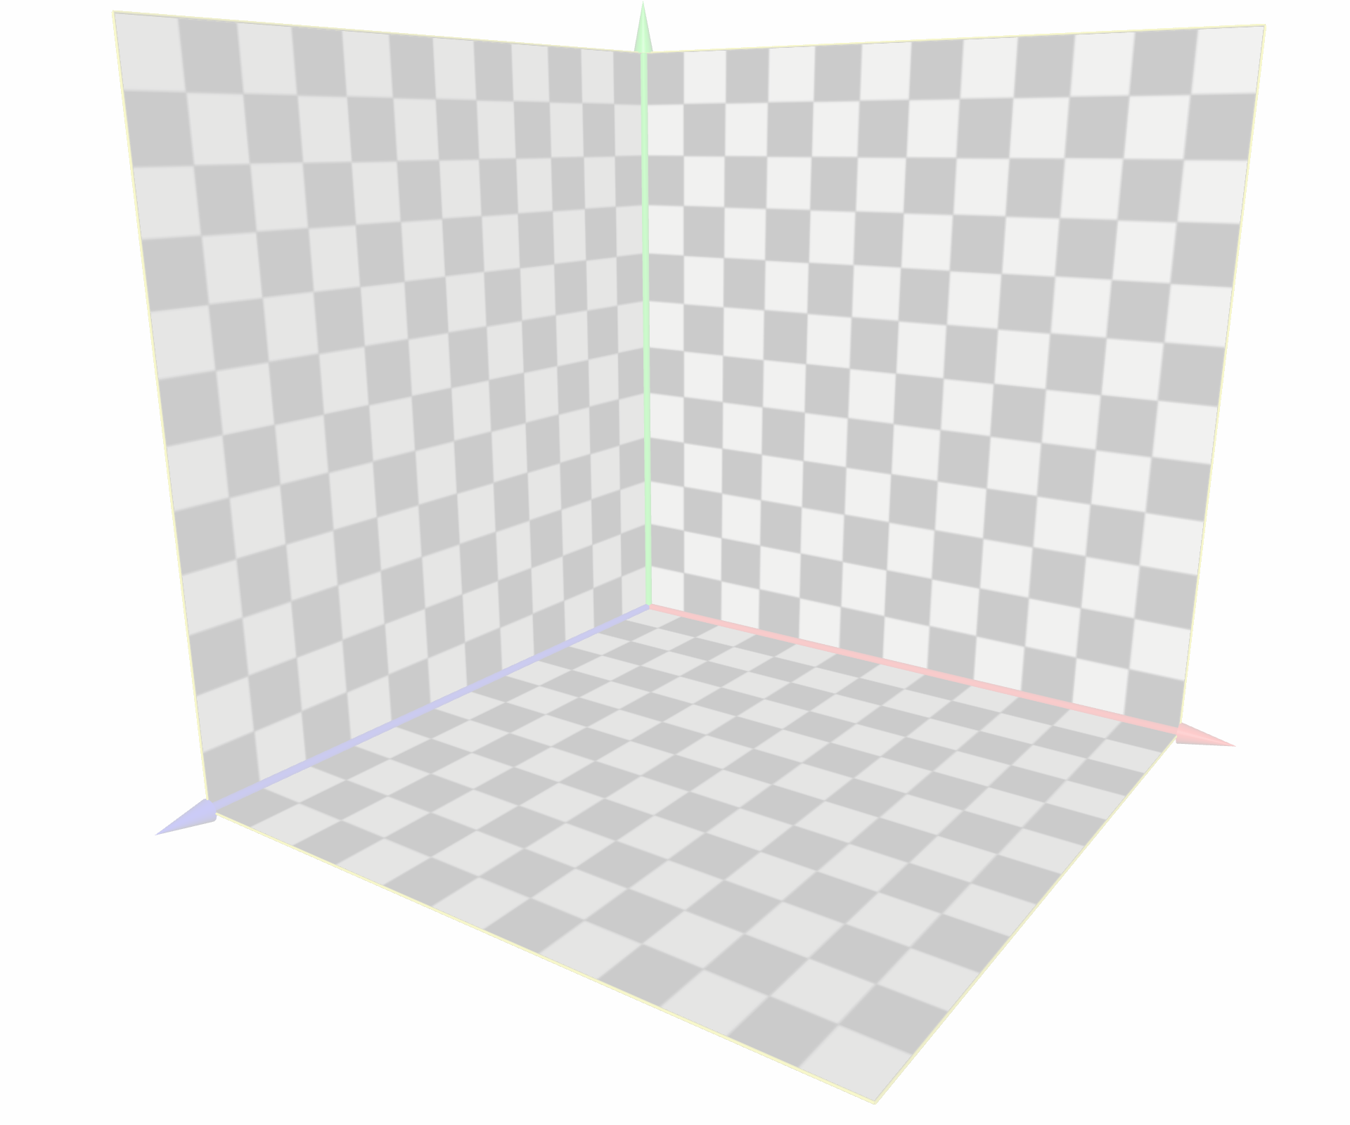
\includegraphics[height=5cm,width=6cm]{images/test/test_normal.png}
	\end{minipage}
}
\subfigure[result - normal]
{
	\begin{minipage}{7cm}
	\centering     
	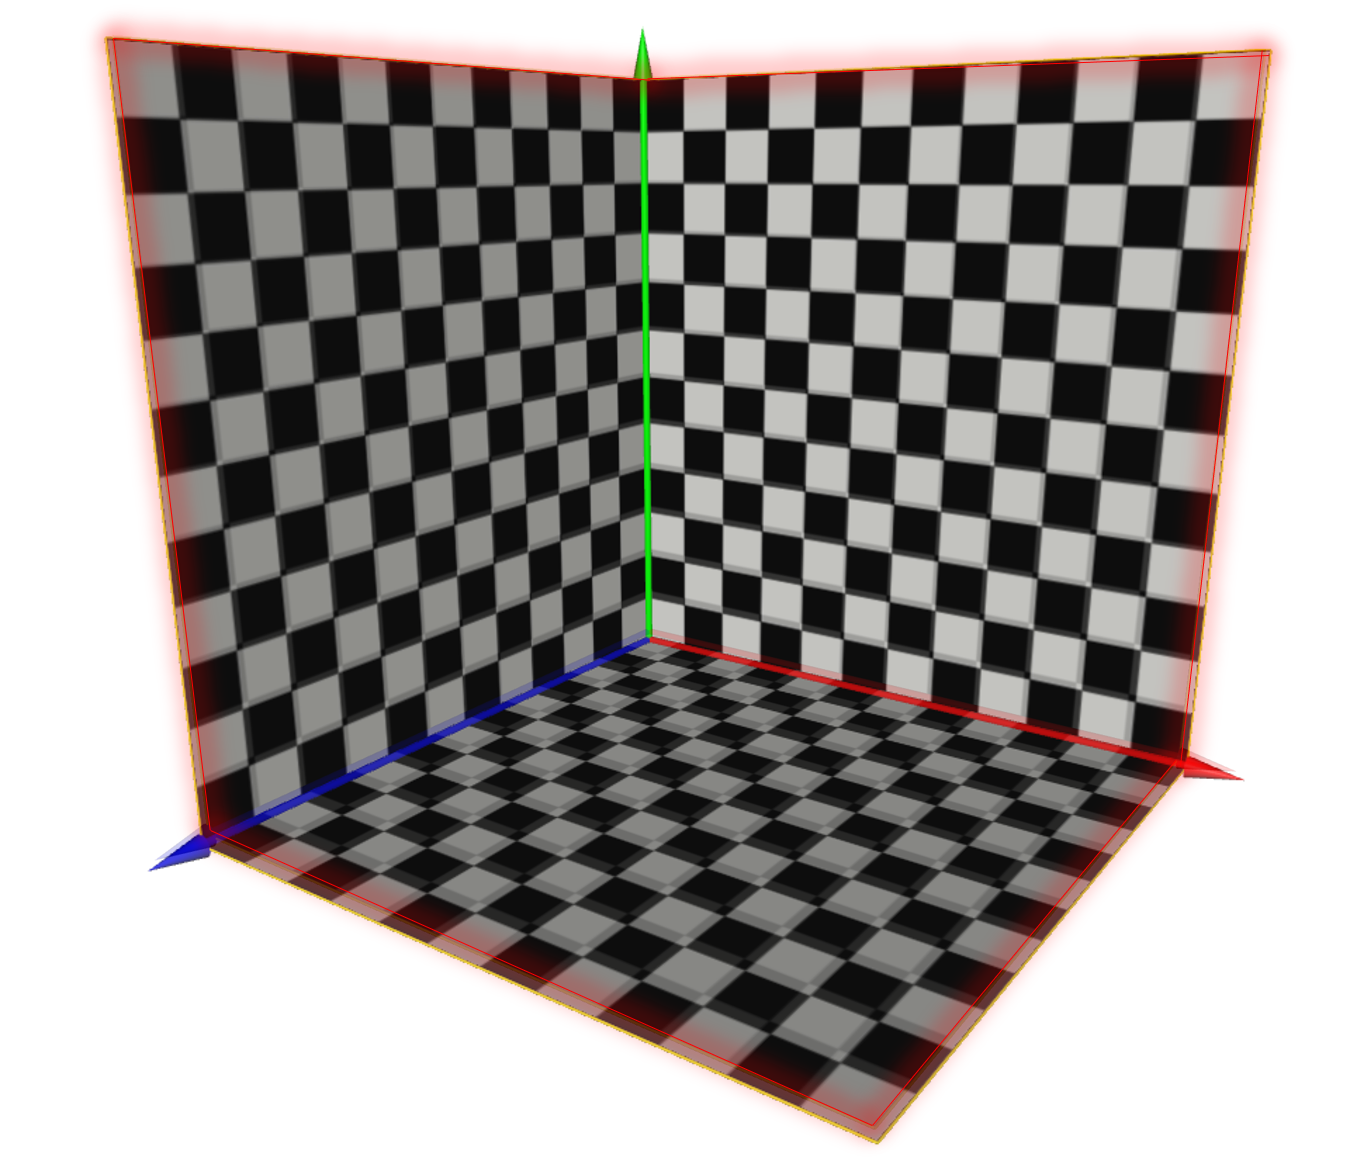
\includegraphics[height=5cm,width=6cm]{images/test/result_normal.png}
	\end{minipage}
}
\caption{Calibration - test\_normal}
\end{figure}

~\\
With such manner, the differences can be intuitively observed. Screenshots of the other two test data sets (noisy, exact) are shown in \textbf{Fig. 2}.
\begin{figure}[htbp]
\centering
\subfigure[test data - noisy]
{
	\begin{minipage}{7cm}
	\centering
	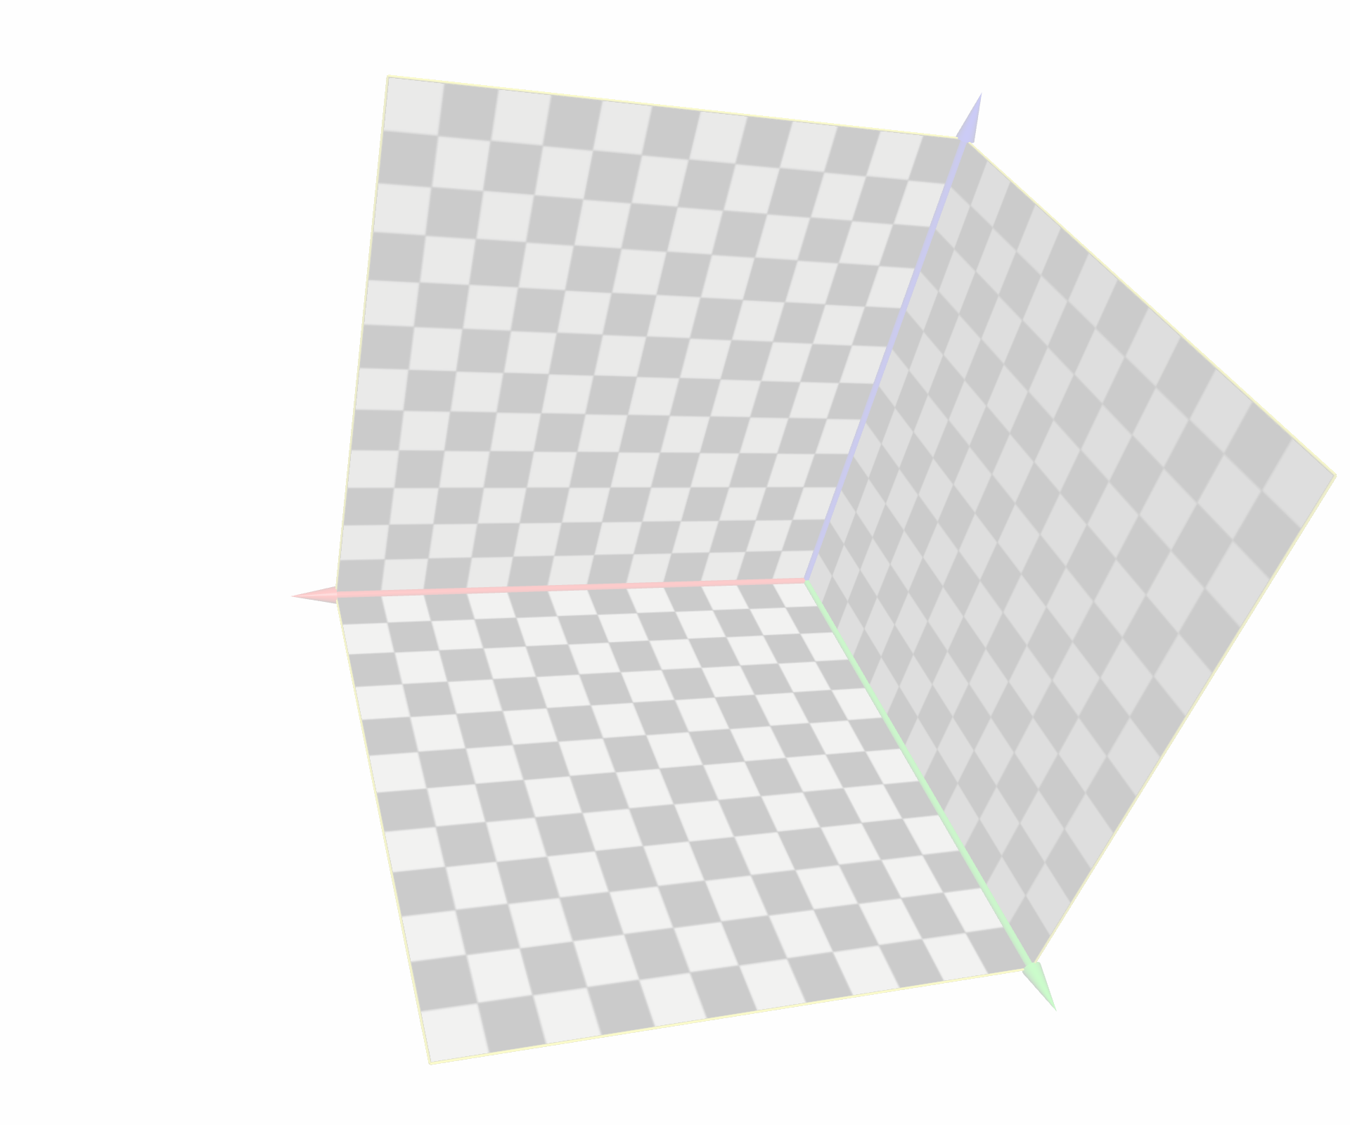
\includegraphics[height=5cm,width=6cm]{images/test/test_noisy.png}
	\end{minipage}
}
\subfigure[result - noisy]
{
	\begin{minipage}{7cm}
	\centering     
	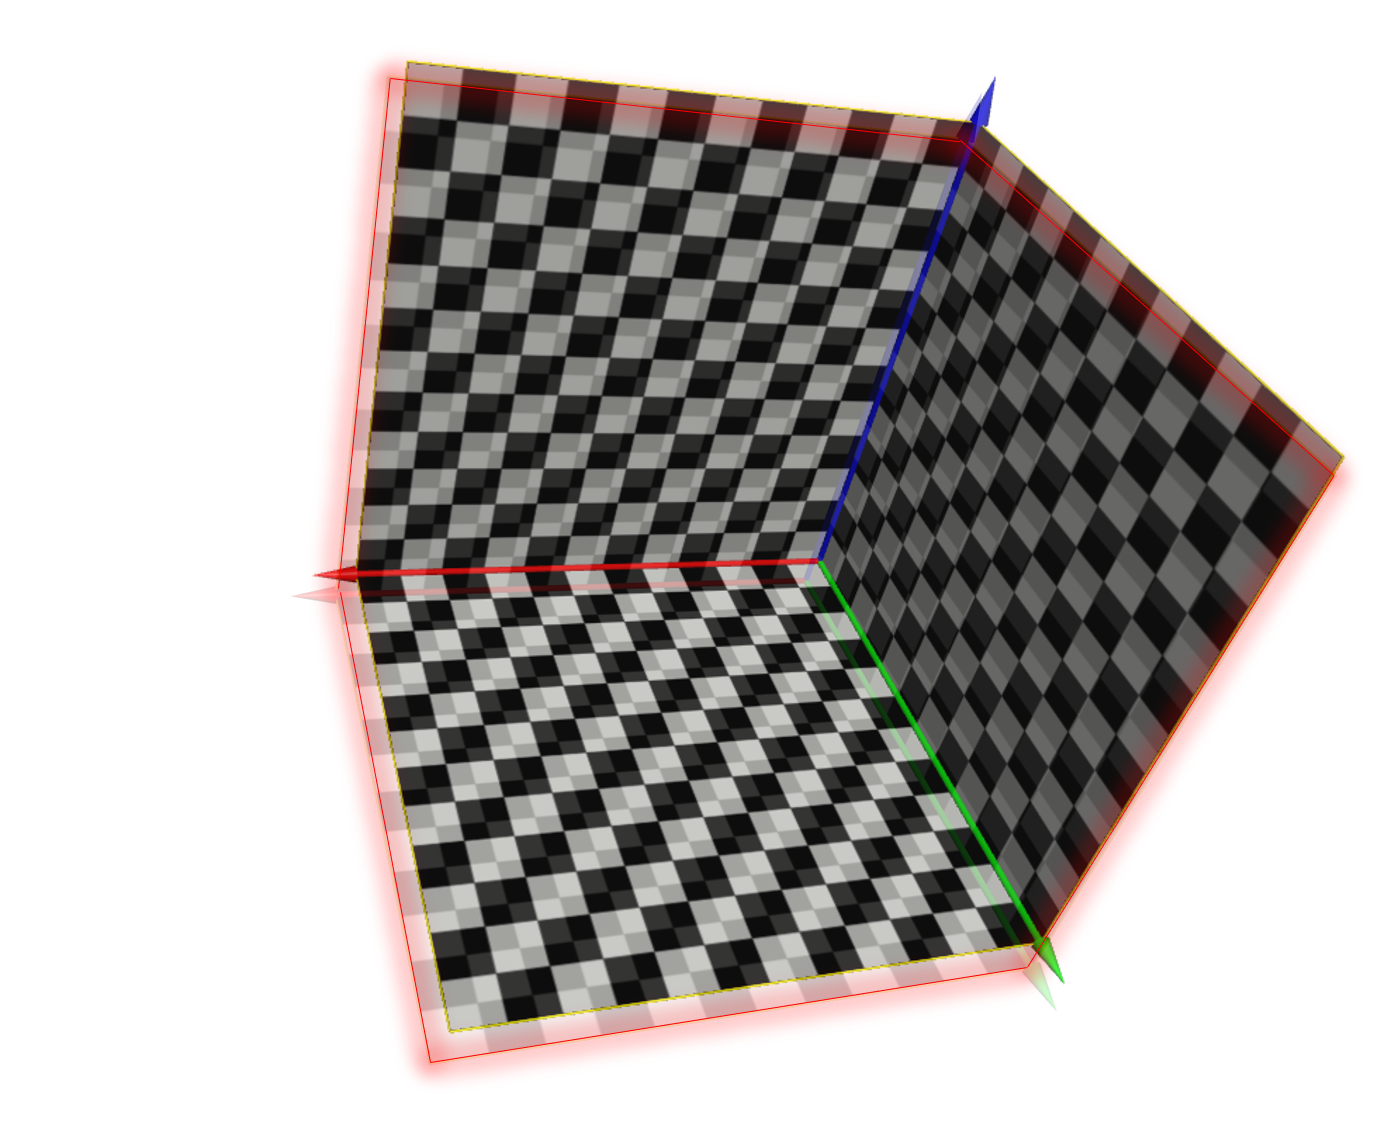
\includegraphics[height=5cm,width=6cm]{images/test/result_noisy.png}
	\end{minipage}
}
\subfigure[test data - exact]
{
	\begin{minipage}{7cm}
	\centering
	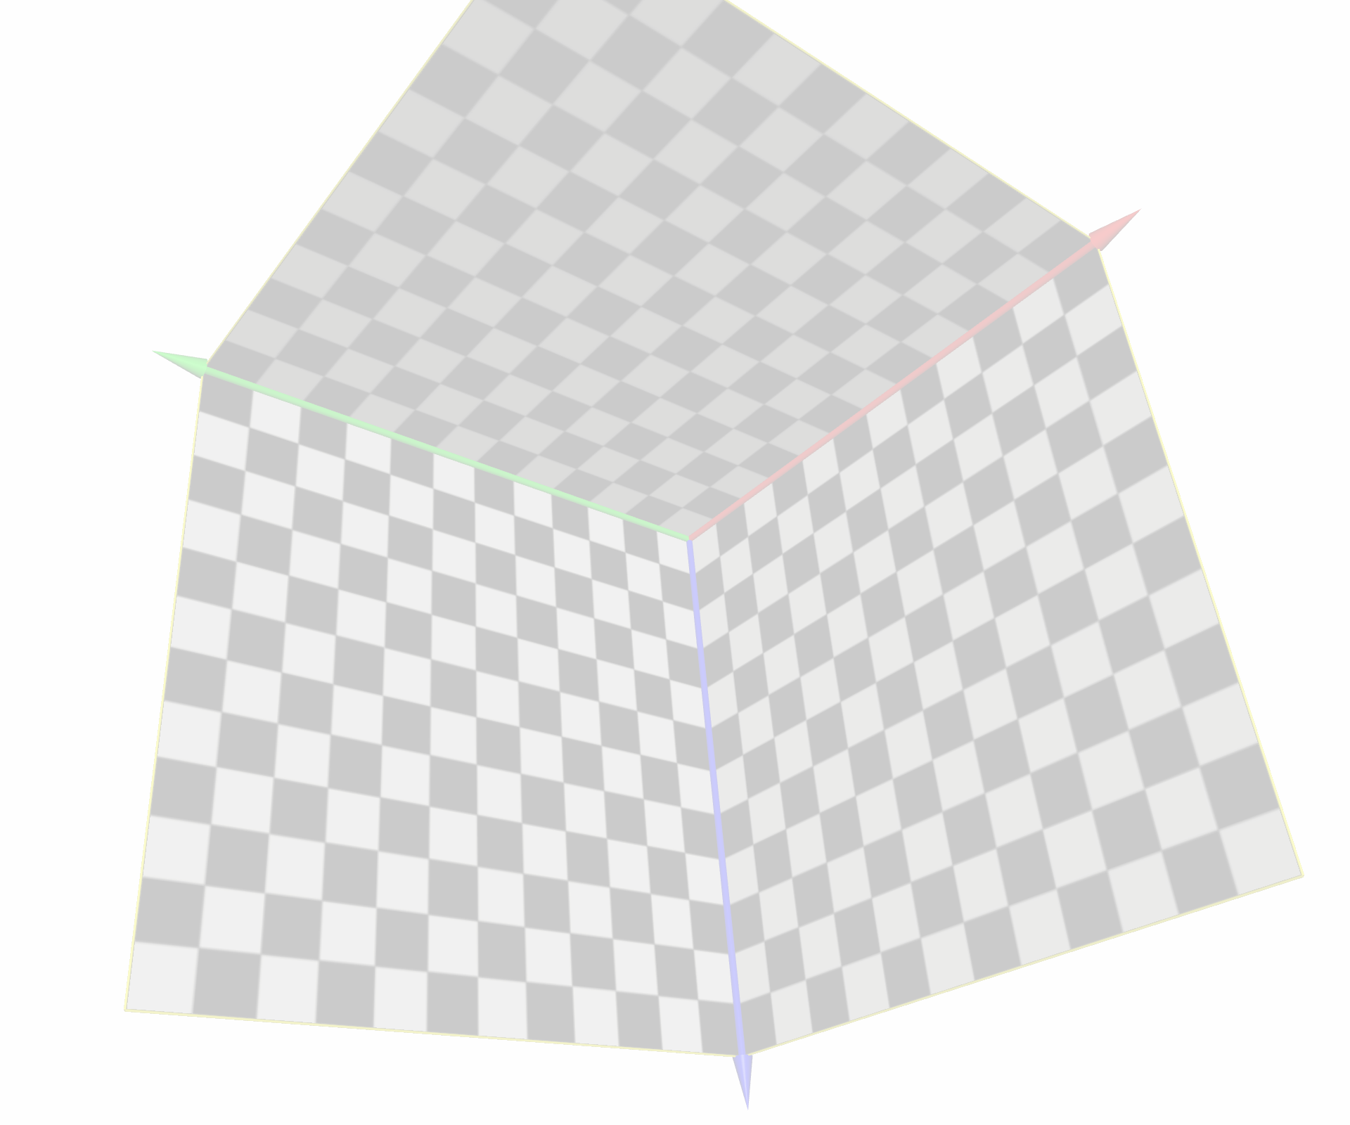
\includegraphics[height=5cm,width=6cm]{images/test/test_exact.png}
	\end{minipage}
}
\subfigure[result - exact]
{
	\begin{minipage}{7cm}
	\centering     
	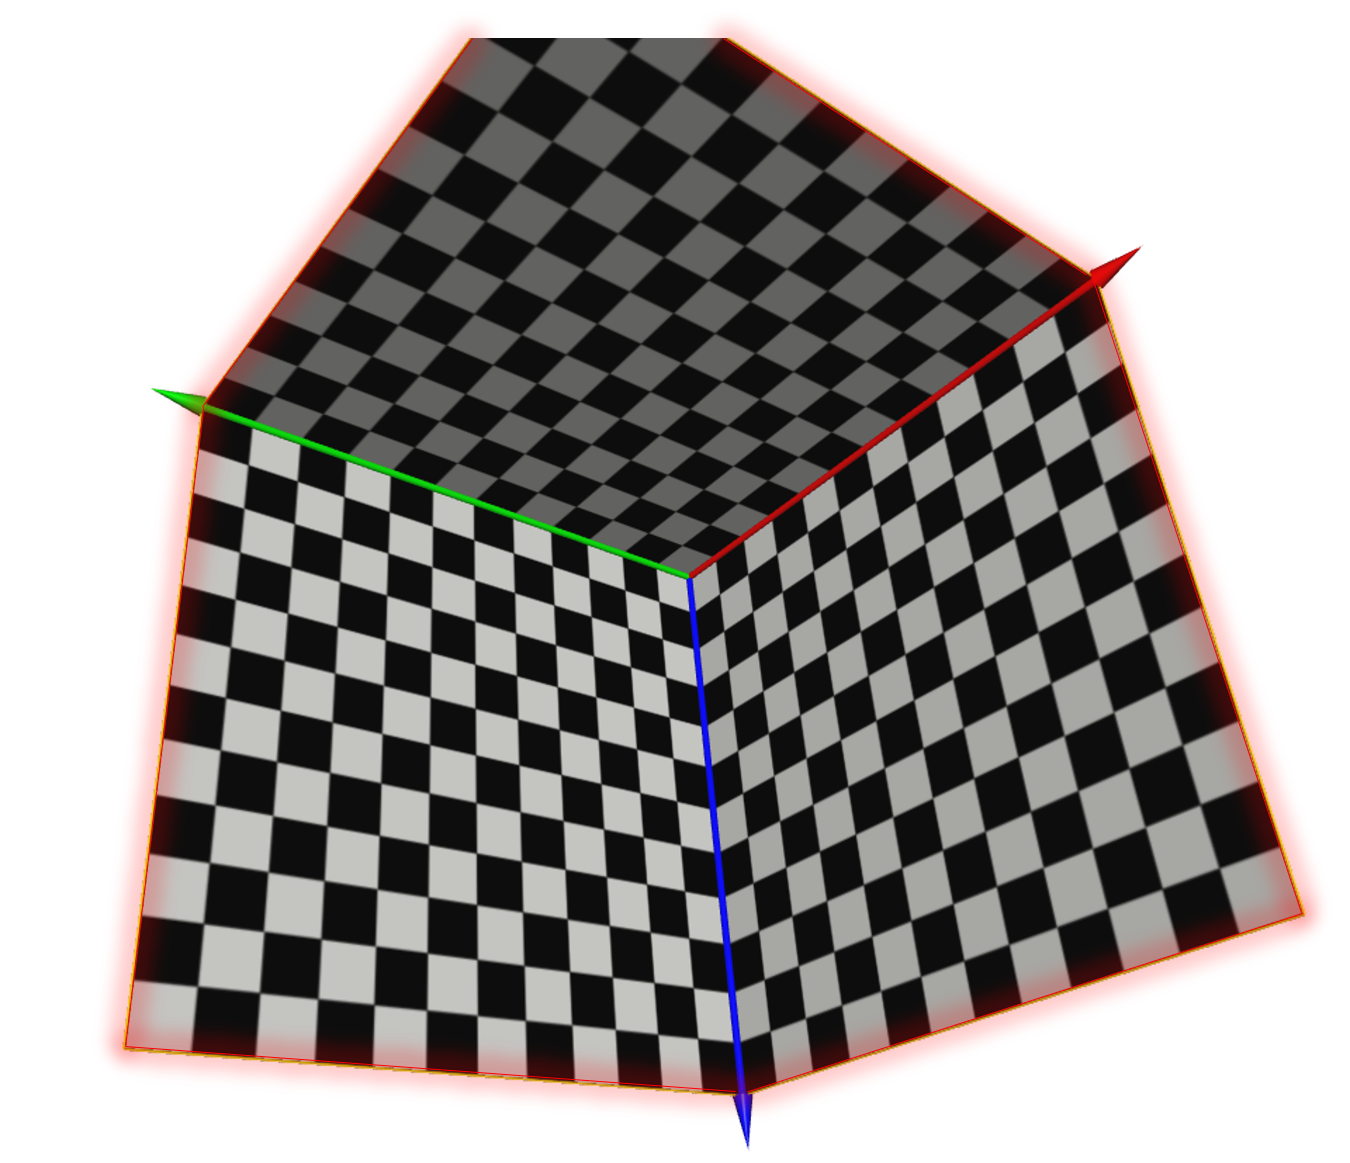
\includegraphics[height=5cm,width=6cm]{images/test/result_exact.png}
	\end{minipage}
}
\caption{Calibration - test\_normal \& exact}
\end{figure}
As is shown in \textbf{Fig. 2}, the deviation reaches the maximum value in the noisy case, which is consistent with the characteristics of the data set itself as well: large errors.
~\\
Although the visualisation comparisons can provide some help in validating the results, a quantitative verification method is essential as it sets out the correctness of the results in numerical terms, see the \textbf{table. 1} below.

\begin{table}[h]\centering
\begin{tabular}{ |c|c| } 
 \hline
 test file & $variance$ \\ 
 \hline
 test\_normal & 0.003 \\ 
 \hline
 test\_noisy & 1.736 \\ 
 \hline
 test\_exact & 8.876e-07 \\ 
 \hline
\end{tabular}
\caption{Calculated results}
\end{table}

In addition to the three known test files, we also created and tested our own modified files:

\begin{itemize}

\item[$\bullet$] \textbf{A1\_9\_points.noisy.txt}

Contains 9 corresponding points (3D/2D), noisy level : noisy.

\item[$\bullet$] \textbf{A1\_9\_points.exact.txt}

Contains 9 corresponding points (3D/2D), noisy level : exact.

\end{itemize}

The visualisation results are shown in \textbf{Fig. 3}.

\begin{figure}[htbp]
\centering
\subfigure[A1\_9\_original]
{
	\begin{minipage}{5cm}
	\centering
	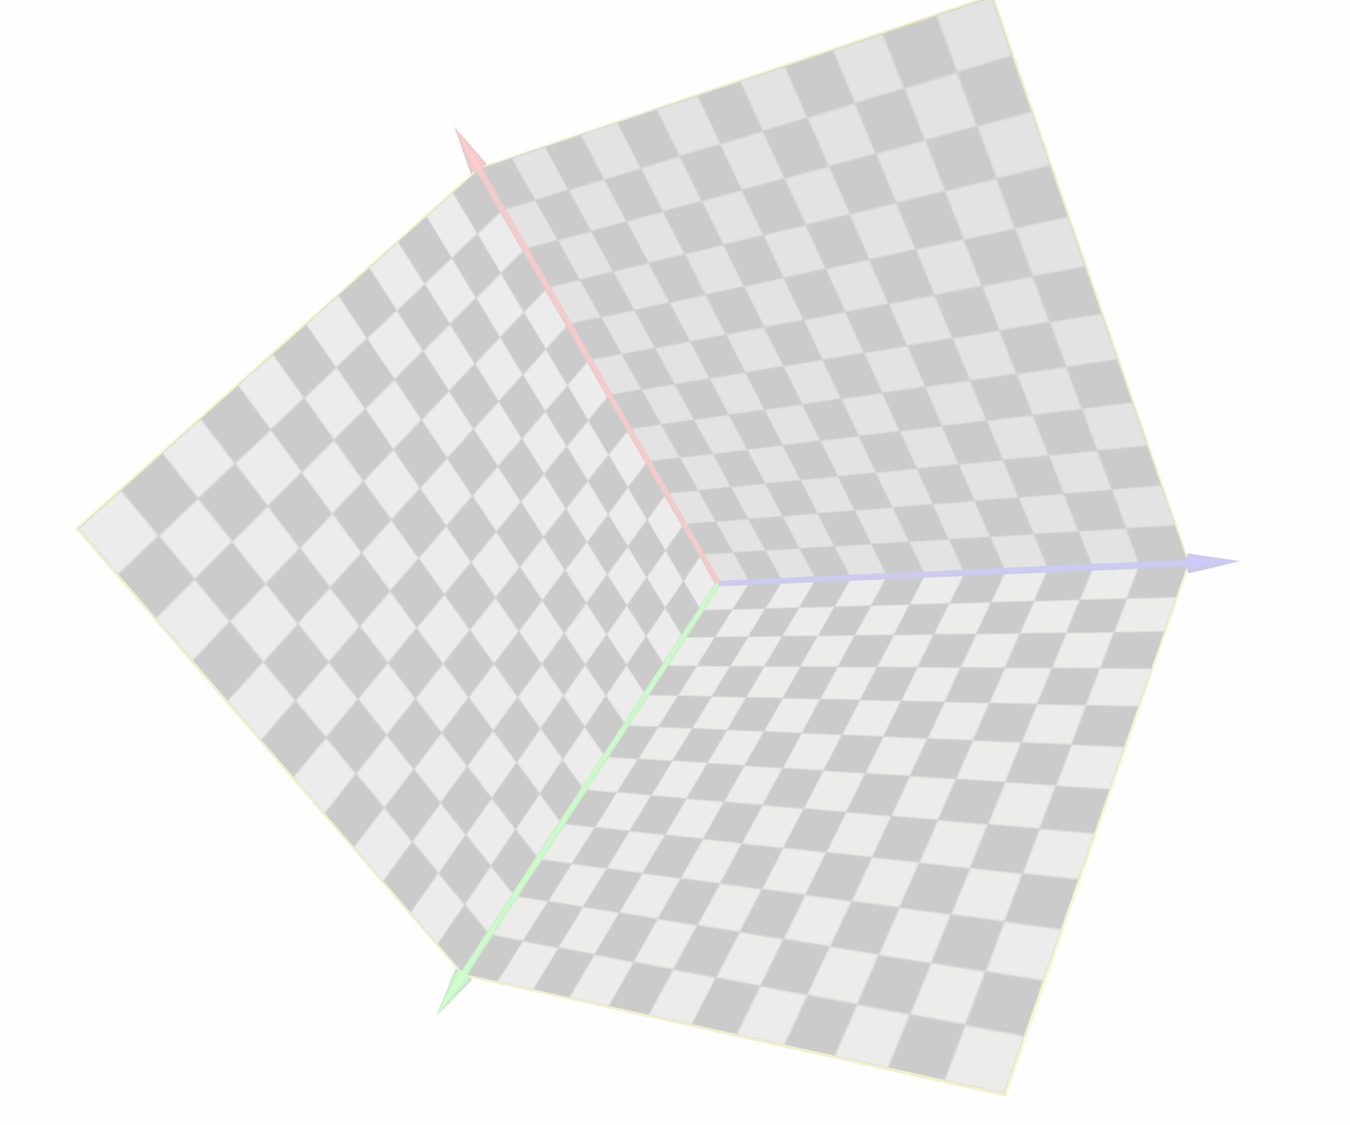
\includegraphics[height=4cm,width=5cm]{images/modified/A1_9_normal.png}
	\end{minipage}
}
\subfigure[A1\_9\_noisy]
{
	\begin{minipage}{5cm}
	\centering     
	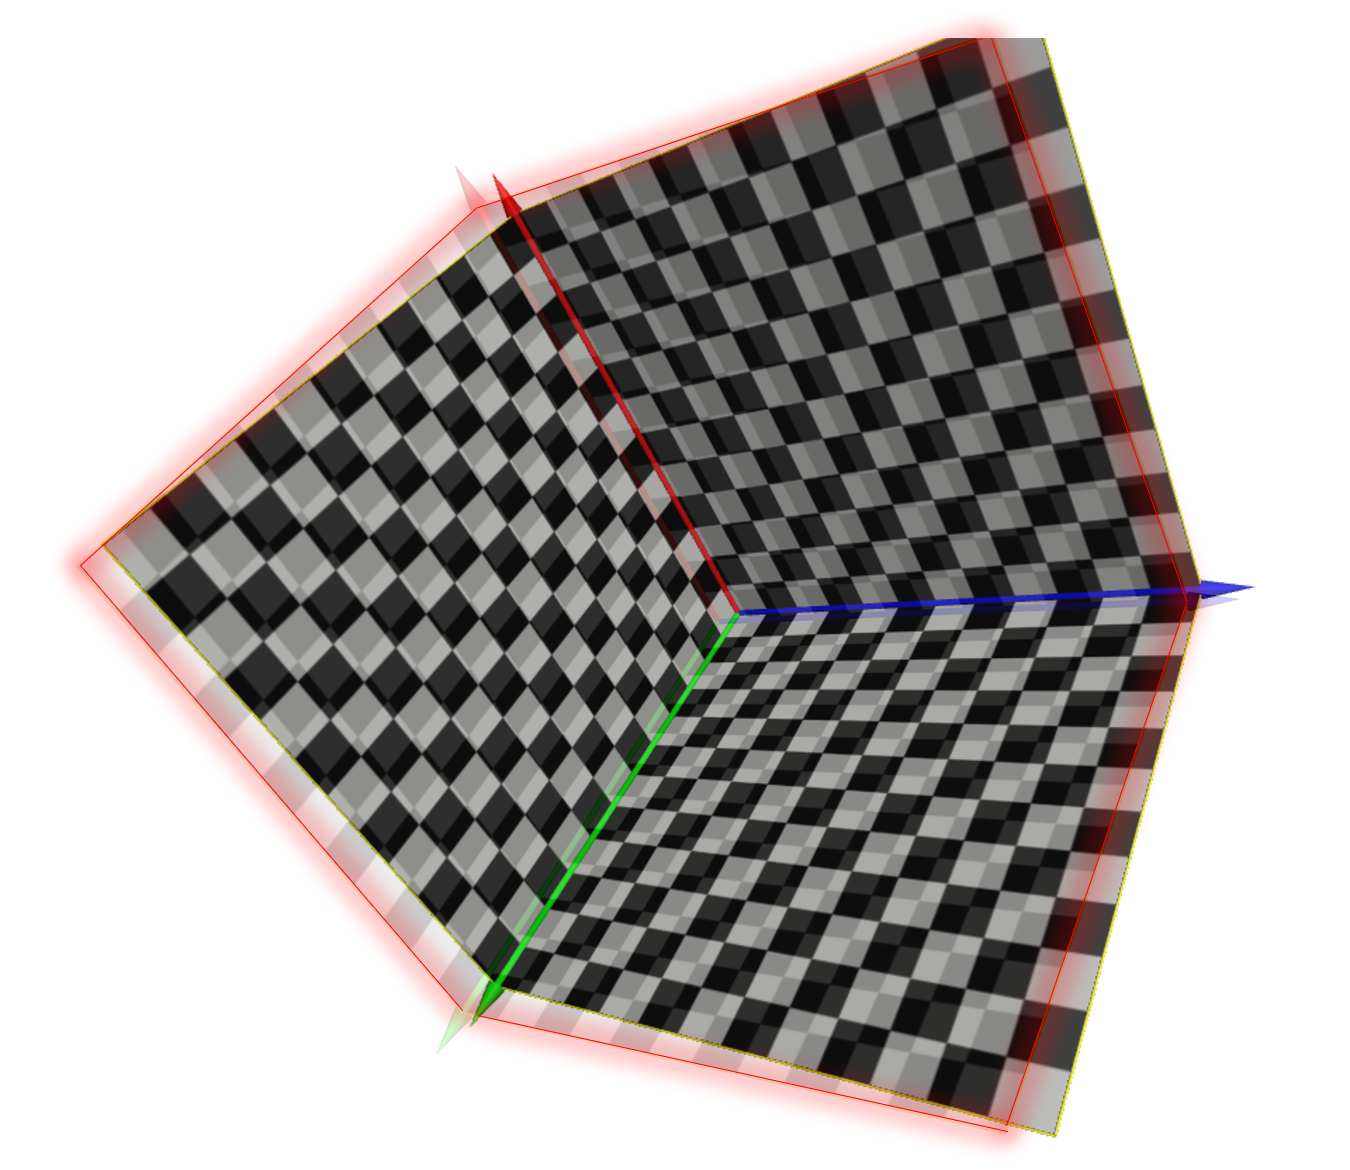
\includegraphics[height=4cm,width=5cm]{images/modified/A1_9_result_normal.png}
	\end{minipage}
}
\subfigure[A1\_9\_exact]
{
	\begin{minipage}{5cm}
	\centering     
	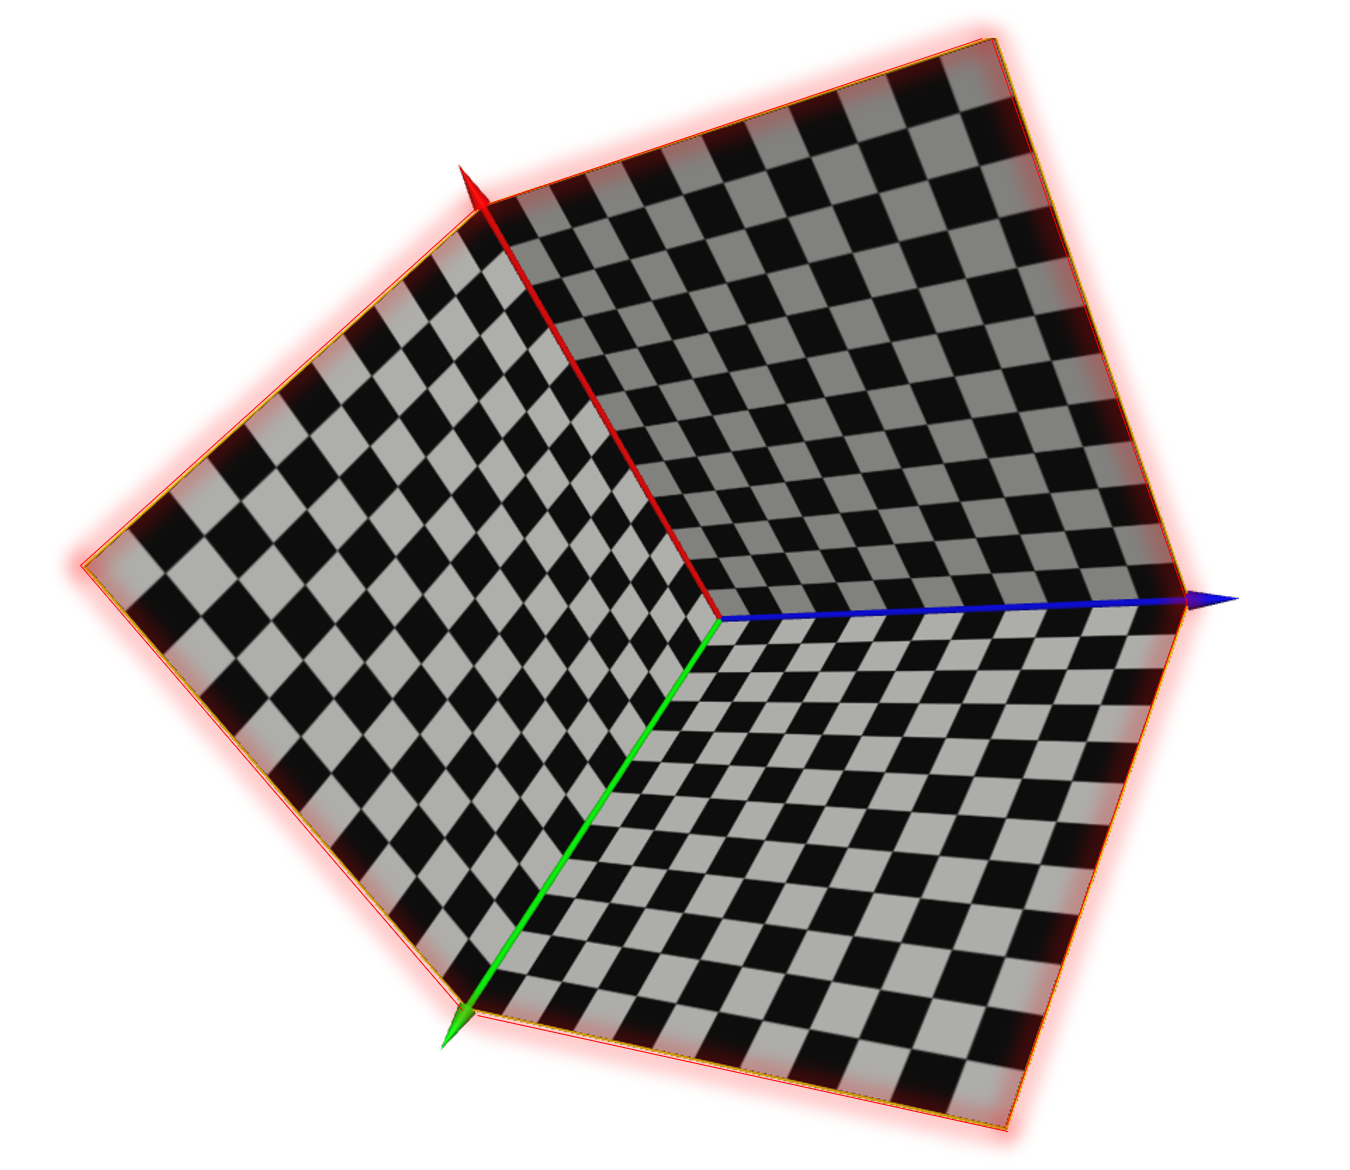
\includegraphics[height=4cm,width=5cm]{images/modified/A1_9_result_exact.png}
	\end{minipage}
}
\caption{Calibration - modified files}
\end{figure}

It should be noted that in \textbf{Fig. 3(c)}, even if we tried to control the image quality as high as possible, the deviations are still quite large. A proper explanation is that it can be tricky when selecting the 2D pixels manually, the details will be described in the analysis part.

As for the $variances$, the $variance$ for   \texthb{A1\_9\_noisy} is approximately 16.139 and for \texthb{A1\_9\_exact} is about 0.099.

\subsection{Performance}
\subsubsection{\small Run time}
We tested the run time of different input files. According to the statistics in \textbf{table. 2}, the run time reaches the maximum when the input file contains the most points.

\begin{table}[h]\centering
\begin{tabular}{ |c|c|c| } 
 \hline
 test file & number of points & run time \\ 
 \hline
 test\_normal & 6 & 35.9821 ms\\ 
 \hline
 test\_noisy & 9 & 60.1746 ms\\ 
 \hline
 test\_exact & 12 & 80.5549 ms\\ 
 \hline
\end{tabular}
\caption{Run time}
\end{table}

It should be noted that the run time can differ due to various reasons, such as CPU type, CPU usage, CPU working frequency and so on. The above results are obtained on a \textit{Windows 10 Intel(R) Core(TM) i7-10875H CPU @ 2.30GHz} platform and they are averages taken after several tests.

\subsubsection{\small Stability}
When testing the effects of the sign of $\rho$, we found if the negative sign(-) was used then we would not be able to zoom in and out after the calibration process even if we could show the camera by pressing key 't'. We couldn't be able to observe the 'inverted' camera and the chessboard from any angle by rotating and translating. Since we lacked the knowledge of the code framework in the limited time, we were unable to understand why this was so. In principle, a change in the symbol of $\rho$ should not affect the position of the chessboard, even if it could affect the status of the calibrated camera. (With the positive sign, we surely can zoom in and out to see the relative position of the calibrated camera and the chessboard)

\subsection{Analysis}
\subsubsection{\small Choosing pixel point}
Choosing pixel point can be tricky due to the resolution of the image we took in the viewer. Please refer to the \textbf{Fig. 4}. The pixels inside the red rectangle can all be considered as potential corresponding 2D point. One important thing is inside each 'pixel cell'(small gray and black rectangle), there can be many pixel points. Therefore choosing the most corresponding point is difficult and thus creating 'exact' input file is hard to achieve. A possible improvement is to traversing all the pixels inside the red rectangle and calculate the average position of these pixels. This average position can be considered as the most corresponding 2D point. In such manner, high quality input files should be obtained.

\subsubsection{\small Calculate variance}
The calculated $variance$ in our case is the sum of squared deviations in $u$ and $v$ direction respectively, which makes $variance$ cumulative and highly sensitive to the errors especially when the deviation is larger than 1. On the other hand, there may be a loss of precision when the computer stores the variables, for example 2.1 may be stored as 2.10000009999, which may also lead to errors in the calculation of the variance. 

\subsubsection{\small Quality}

The quality mainly depends on the quality of the input files(such as noisy level, the number of correspondences). Overall if the quality of the input data sets is high and the number of 3D/2D correspondences is big enough, the results will be most likely reliable.

\begin{figure}[htbp]
\centering
\subfigure[Choosing pixel - 1]
{
	\begin{minipage}{7cm}
	\centering
	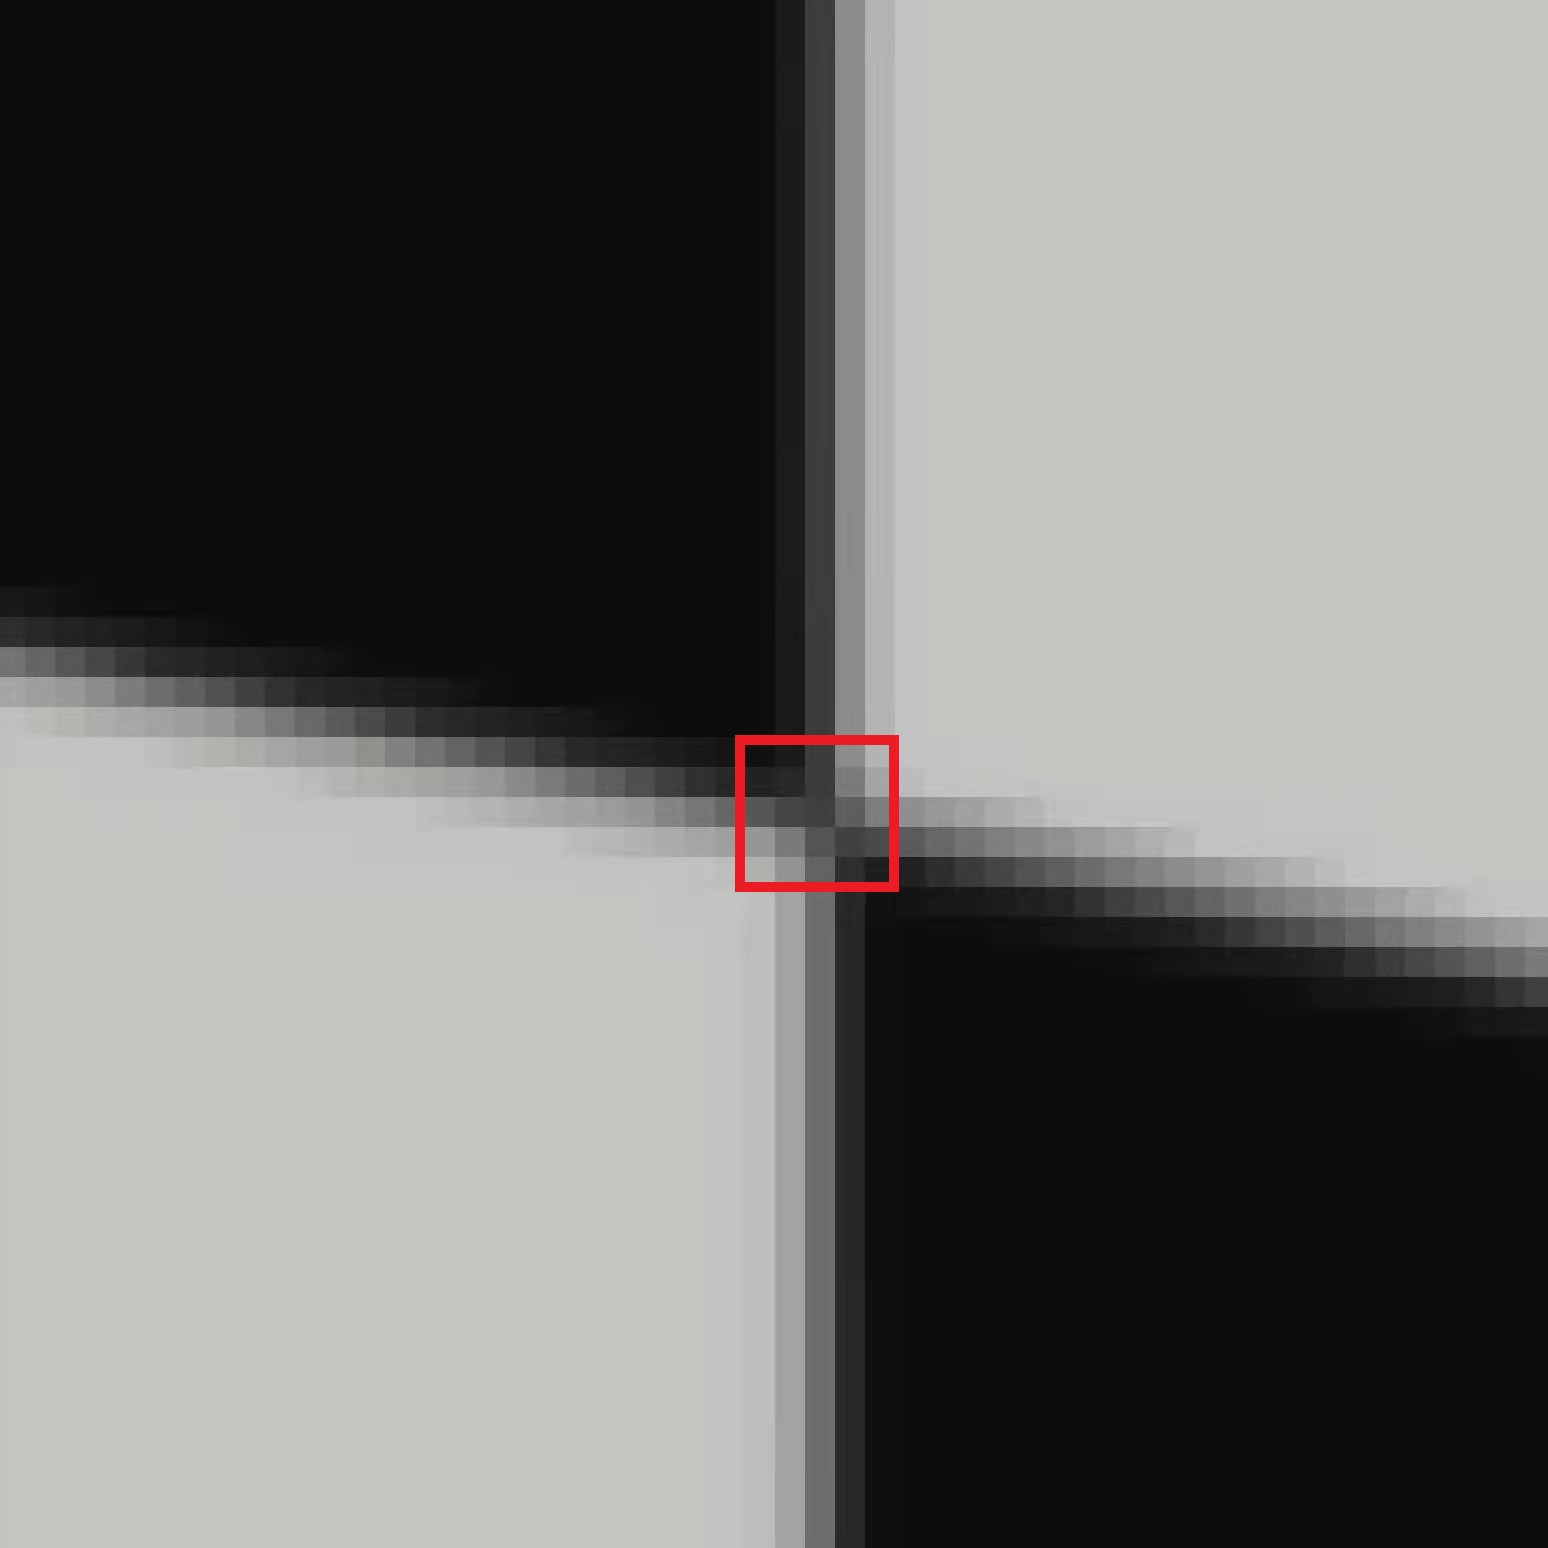
\includegraphics[height=5cm,width=6cm]{images/pixel/pixel1.jpg}
	\end{minipage}
}
\subfigure[Choosing pixel - 2]
{
	\begin{minipage}{7cm}
	\centering     
	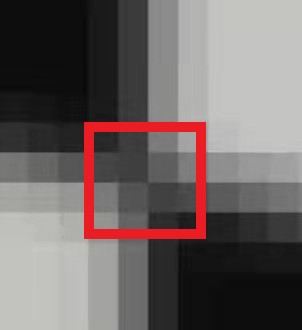
\includegraphics[height=5cm,width=6cm]{images/pixel/pixel2.jpg}
	\end{minipage}
}
\caption{Choosing Pixel Point}
\end{figure}

\section{Devision of work}

In order to fully understand the calibration method, we implemented the algorithm respectively and then merge the code. For the report, \textit{Yitong} provided the modified input files and wrote the Methodology part. \textit{Leo} and \textit{Fengyan} wrote the Introduction and Result \& Analysis parts.

~\\
Our GitHubs:

Leo's \href{https://github.com/leowhk/A1_calibration}{GitHub}.

Yitong's \href{https://github.com/YitongXia/camera-calibration}{GitHub}.

Our solutions are located \href{https://github.com/SEUZFY/Camera_Calibration}{here(merged code)}.

\section{Reference}
[1] \  David Forsyth, Jean Ponce. Computer Vision: A Modern Approach. (Second edition). Prentice Hall, pp.792, 2011, 978-0136085928. \href{https://hal.inria.fr/hal-01063327}{⟨hal-01063327⟩}

[2] \  GEO1016 course page. \href{https://3d.bk.tudelft.nl/courses/geo1016/index.html}{geo1016}

\end{document}